 \documentclass[12pt]{article}
\pagestyle{myheadings}
\usepackage{graphicx}
\usepackage{listings}


%Enter your name, the portfolio problem number, and the draft number.
\title{CMPE211:combinatorial algorithm Designing Against an Adversary Assignment}
\author{Weiting Zhan}

%Enter your name, the portfolio problem number, and the draft number.  This will be a heading on pages after the first page.
\markright{CMPE211: Designing Against an adversary Assignment}


\usepackage{amsmath,amssymb,amsthm,amsfonts,graphics}

%The following commands allow us to typeset theorems, propositions, definitions, etc.
\theoremstyle{plain}
\newtheorem{theorem}{Theorem}
\newtheorem{lemma}[theorem]{Lemma}
\newtheorem{corollary}[theorem]{Corollary}
\newtheorem{proposition}[theorem]{Proposition}
\newtheorem*{definition}{Definition}

\renewcommand{\qedsymbol}{\ensuremath{\blacksquare}}


\begin{document}
\maketitle

%Enter your email address.
\begin{center}
\textbf{Email address: wzhan83@ucsc.edu}
\end{center}


\section{Given an algorithm to find the median of five keys with only six comparisons in worst case.}


The strategy of finding the medium of  $<a,b,c,d,e>$ are described below. The decision rule is that after each comparison , the permutation of results are balanced.











The detail of explanation are shown below. The higher the nodes, the bigger the value. Each step, compare the blue nodes. The yellow node is the medium of the 5 nodes.


\\1.  Start a merge sort with the first 4 elements and order each pair (a,b) (c,d) (2 comparisons) 

2.  Compare the two higher ones of each pair.i.e. compare (b,d) (3rd comparison)  

3.  compare the 5th elements to the number without a pair. compare (c,e)(4th comparison) 

4.  Compare the left children and right children of the root. i.e (b,c) (5th comparison) 


5.  Compare the left children of the second higher nodes and the right children of the second higher nodes. The bigger one is the medium.(6th comparison) 

\begin{figure}[h]
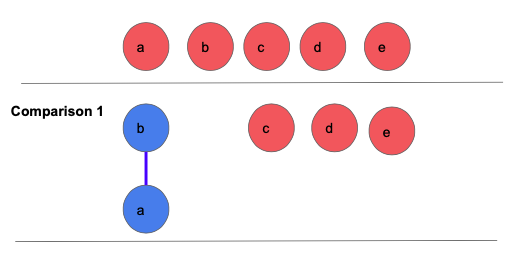
\includegraphics[width=12cm]{1.png}
\centering
\caption{The 1st comparison}
\label{BF}
\end{figure}

\begin{figure}[h]
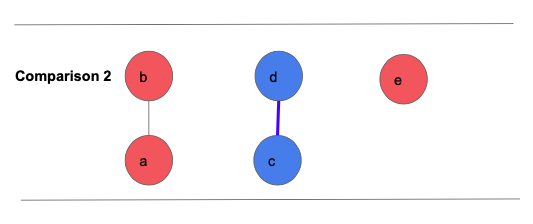
\includegraphics[width=12cm]{2.png}
\centering
\caption{The 2nd comparison}
\label{BF}
\end{figure}

\begin{figure}[h]
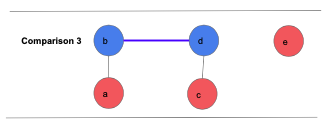
\includegraphics[width=12cm]{3.png}
\centering
\caption{The 3rd comparison}
\label{BF}
\end{figure}

\begin{figure}[h]
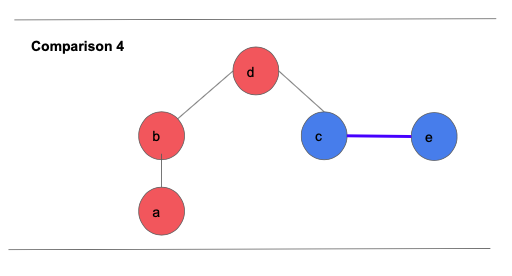
\includegraphics[width=12cm]{4.png}
\centering
\caption{The 4th comparison}
\label{BF}
\end{figure}

\begin{figure}[h]
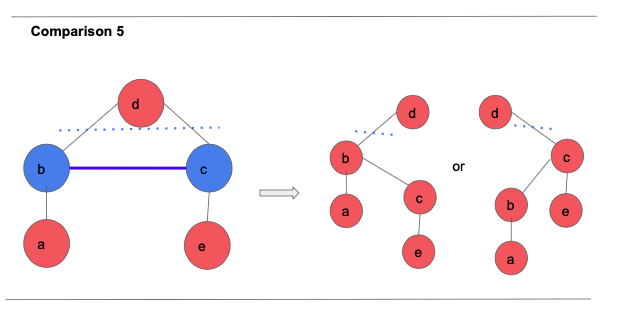
\includegraphics[width=12cm]{5.png}
\centering
\caption{The 5th comparison}
\label{BF}
\end{figure}

\begin{figure}[h]
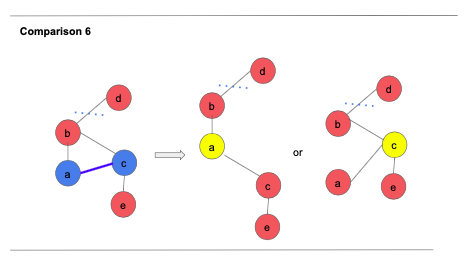
\includegraphics[width=12cm]{6.png}
\centering
\caption{The 6th comparison}
\label{BF}
\end{figure}



\clearpage

\section{Given an algorithm to sort five keys with only seven comparisons in the worst case.}



1. Make 2 groups (A,B) (C,D)

2. Compare A to B and C to D, suppose $A<B$ (compare operation 1) and $C<D$ (compare operation 2). 

3. Compare B to D, suppose $B>D$ (compare operation 3).

4. Sort E into B-D-C.
    
    compare E with the middle of the 3 elements(B-D-C), i.e D (compare operation 4):
    
    
    if $E> D$:
        
        compare E to B (compare operation 5):
        
        if $E > B $ : E-B-D-C
        
        if $E < B$: B-E-D-C
    
    if $E <D$:
        compare E to C:
        if $E > C$: B-D-E-C
        if $E < C$: B-D-C-E

5. Sort A into B's right children $<D,C,E>$ or $<D,E,C>$ or $<E,D,C>$ or $<B,D,C>$. As shown in Figure 11.
    
    This can be done with two comparisons as shown in step 4 (compare operation 6,7), for a total of seven.
\begin{figure}[h]
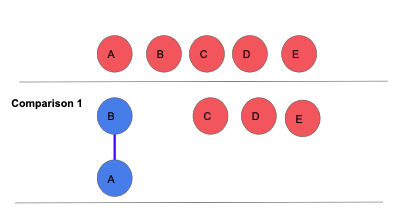
\includegraphics[width=12cm]{21.png}
\centering
\caption{1st comparison}
\label{BF}
\end{figure}


\begin{figure}[h]
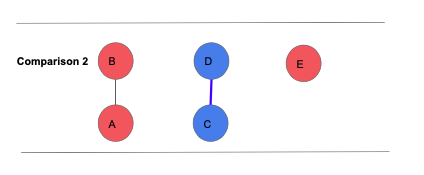
\includegraphics[width=12cm]{22.png}
\centering
\caption{2nd comparison}
\label{BF}
\end{figure}


\begin{figure}[h]
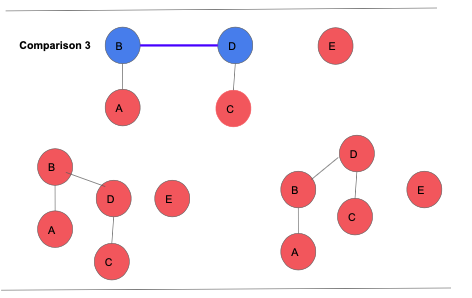
\includegraphics[width=12cm]{23.png}
\centering
\caption{3rd comparison}
\label{BF}
\end{figure}

\begin{figure}[h]
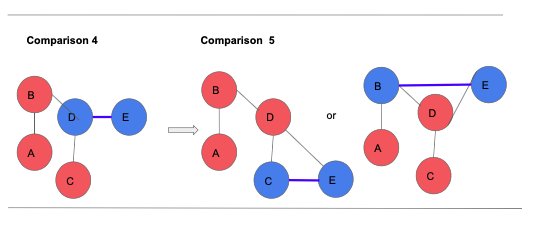
\includegraphics[width=12cm]{24.png}
\centering
\caption{4th and 5th comparison}
\label{BF}
\end{figure}

\begin{figure}[h]
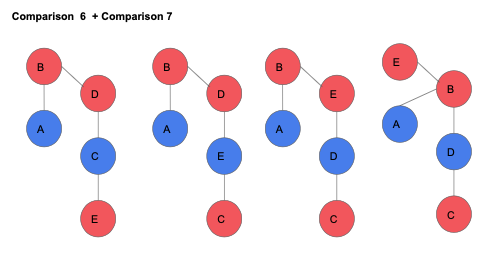
\includegraphics[width=12cm]{25.png}
\centering
\caption{6th and 7th comparison}
\label{BF}
\end{figure}



\end{document}


